\documentclass[12pt]{article}
\usepackage{enumerate}
\usepackage{notes}

\begin{document}
\title{Part A Linear Algebra}
\maketitle

\section*{Sheet 1}
\subsection*{} % 1
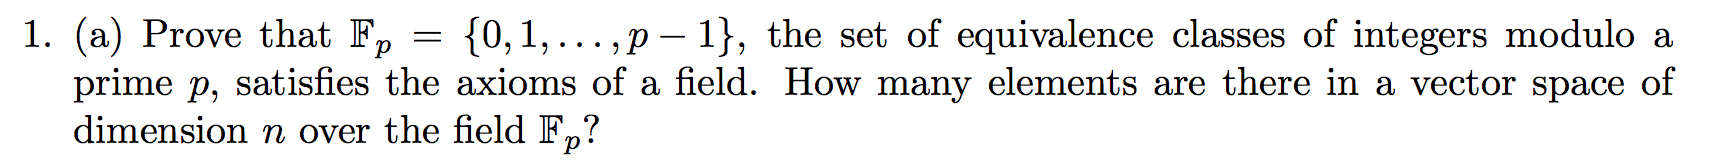
\includegraphics[width=450pt]{img/linear-algebra-a0-1-1-a.png}\\
\begin{mdframed}
  Let $a, b, c \in \Z$ with $0 \leq a < p, ~~ 0 \leq b < p, ~~ 0 \leq c < p$.

  Let $\bar a, \bar b, \bar c \in \F$ be equivalence classes of integers modulo $p$.

  The field axioms are listed below, together with proof that they hold for $\F_p$.
  \begin{enumerate}
  \item \textbf{Additive axioms}\\
    Define $\bar a + \bar b := \bar{a + b}$, then:
    \begin{enumerate}
    \item \textit{Existence of identity}: $\bar 0$ is the identity since
      $\bar a + \bar 0 = \bar{a + 0} = \bar{a}$ for all $\bar a \in \F_p$.
    \item \textit{Existence of inverses}: $(\bar a)^\1 = \bar{-a}$ since
      $\bar a + \bar{-a} = \bar{a + -a} = \bar{0}$ for all $a \in \F_p$.
    \item \textit{Commutativity}:
      $\bar a + \bar b = \bar{a + b} = \bar{b} + \bar{a}$ for all $a, b \in \F_p$.
    \item \textit{Associativity}:
      $\bar a + (\bar b + \bar c) = \bar a + \bar {b + c} = \bar{a + b + c} =
      \bar{a + b} + \bar{c} = (\bar a + \bar b) + \bar{c}$.
    \end{enumerate}
  \item \textbf{Multiplicative axioms}\\
    Define $\bar a ~ \bar b := \bar{ab}$, then:
    \begin{enumerate}
    \item \textit{Existence of identity}: $\bar 1$ is the identity since
      $\bar a \bar 1 = \bar{a\cdot 1} = \bar{a}$ for all $\bar a \in \F_p$.
    \item \textit{Existence of inverses for everything except additive
        identity}: We need to show that for all
      $\bar a \in \F_p \setminus \{\bar 0\}$ there exists $\bar b \in \F_p$
      such that $\bar a ~ \bar b = \bar 1$. \red{TODO: I couldn't think how to
        show this. I eventually allowed myself to google a little which brought
        up people pointing to the fact that since $a$ and $p$ are coprime,
        there exist $n, m$ such that $an + pm = 1$. Haven't thought about what
        to do with that yet.}
    \item \textit{Commutativity}:
      $\bar a ~ \bar b = \bar{ab} = \bar{b} ~ \bar{a}$ for all $a, b \in \F_p$.
    \item \textit{Associativity}:
      $\bar a (\bar b \bar c) = \bar a + \bar {bc} = \bar{abc} =
      \bar{ab}~\bar{c} = (\bar a ~ \bar b) \bar{c}$.
    \end{enumerate}
  \item \textbf{Distributive axiom}
    \begin{enumerate}
    \item \textit{Multiplication distributes over addition}: $\bar a (\bar b + \bar c) = \bar a (\bar{b + c}) = \bar{a(b+c)} = \bar{ab +
      ac} = \bar{ab} + \bar{ac} = \bar{a}~\bar{b} + \bar{a}~\bar{c}$
    \end{enumerate}
  \end{enumerate}

There are $p^n$ elements in a vector space of dimension $n$ over the field $\F_p$.
\end{mdframed}
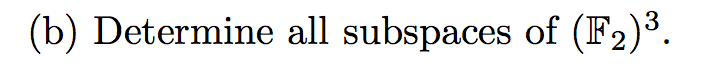
\includegraphics[width=250pt]{img/linear-algebra-a0-1-1-b.png}
\begin{mdframed}
  \textit{Remark}: This is like the 8 vectors that form the unit cube in
  $\R^3$, except that when extended beyond the cube by vector addition or
  scalar multiplication they ``wrap around''.

  Note that
  \begin{align*}
    (\F_2)^3 = \{&\bar 0, \bar 1\}^3\\
             = \{&(\bar 0, \bar 0, \bar 0),\\
                 &(\bar 0, \bar 0, \bar 1),\\
                 &(\bar 0, \bar 1, \bar 0),\\
                 &(\bar 0, \bar 1, \bar 1),\\
                 &(\bar 1, \bar 0, \bar 0),\\
                 &(\bar 1, \bar 0, \bar 1),\\
                 &(\bar 1, \bar 1, \bar 0),\\
                 &(\bar 1, \bar 1, \bar 1)\}.
  \end{align*}
  The set of subspaces of $(\F_2)^3$ is
  \begin{align*}
    &\{\{(\bar 0, \bar 0, \bar 0)\}\} ~~~~~~~~~~~~~~~~~~~~~ \cup\\
    &\{\{(\bar 0, \bar 0, \bar 0), x\} ~|~ x \in (\F_2)^3\} ~~~ \cup\\
    &\{\{(\bar 0, a, b) ~|~ a, b \in \F_2\}\}  ~~~~~~~ \cup\\
    &\{\{(a, \bar 0, b) ~|~ a, b \in \F_2\}\}  ~~~~~~~ \cup\\
    &\{\{(a, b, \bar 0) ~|~ a, b \in \F_2\}\}  ~~~~~~~ \cup\\
    &\{(\F_2)^3\}.
  \end{align*}
\end{mdframed}


\subsection*{} % 2

\includegraphics[width=450pt]{img/linear-algebra-a0-1-2.png}\\
\begin{mdframed}
We need to:
\begin{enumerate}
\item \textbf{\textit{Exhibit a proper subspace $S[x] \subset \R[x]$ and a bijection $f:\R[x] \to S[x]$}}\\\\
  Let $a_i \in \R$ for $i = 0, 1, 2, \ldots$ so that
  $\R[x] = \{a_0 + a_1x^1 + a_2x^2 + \ldots\}$.

  Define $S[x] = \{0 + a_1x^1 + a_2x^2 + a_3x^3 + \ldots\}$, i.e. the restriction
  of $\R[x]$ to those polynomials that have constant term zero.

  $S[x]$ is a proper subspace of $\R[x]$ since it contains the zero polynomial,
  and is closed under addition and scalar multiplication.

  Define $f: \R[x] \to S[x]$ where
  $f(a_0 + a_1x^1 + a_2x^2 + \ldots) = 0 + a_0x^1 + a_1x^2 + a_2x^3 + \ldots$.

  $f$ is clearly injective, since if $f(r(x)) = f(r'(x))$ then their
  coefficients $a_0, a_1, \ldots$ are the same and hence $r(x) = r'(x)$.

  Also, $f$ is clearly surjective since if
  $s(x) = a_1x^1 + a_2x^2 + a_3x^3 + \ldots$ then
  $s(x) = f(a_1 + a_2x^1 + a_3x^2 + \ldots)$.

\item \textbf{\textit{Prove that $f$ preserves addition}}\\\\
  Let $a_i,b_i \in \R$ for $i = 0, 1, 2, \ldots$

  Let $r(x) = a_0 + a_1x^1 + a_2x^2 + \ldots$ and $r'(x) = b_0 + b_1x^1 + b_2x^2 + \ldots$.

  Then
  \begin{align*}
    f\Big(r(x) + r'(x)\Big)
    &= f\Big((a_0 + b_0) + (a_1 + b_1)x^1 + (a_2 + b_2)x^2 + \ldots\Big)\\
    &= 0 + (a_0 + b_0)x^1 + (a_1 + b_1)x^2 + (a_2 + b_2)x^3 + \ldots\\
    &= \Big(0 + a_0x^1 + a_1x^2 + a_2x^3 + \ldots \Big) \\
    &+ \Big(0 + b_0x^1 + b_1x^2 + b_2x^3 + \ldots \Big) \\
    &= f\Big(r(x)\Big) + f\Big(r'(x)\Big).
  \end{align*}

  \begin{align*}
  \end{align*}

\item \textbf{\textit{Prove that $f$ preserves scalar multiplication}}
  \begin{align*}
    f\Big(\lambda r(x)\Big)
    &= f\Big(\lambda a_0 + \lambda a_1x^1 + \lambda a_2x^2 + \ldots \Big) \\
    &= 0 + \lambda a_0x^1 + \lambda a_1x^2 + \lambda a_2x^3 + \ldots \\
    &= \lambda(0 + a_0x^1 + a_1x^2 + a_2x^3 + \ldots) \\
    &= \lambda f\Big(r(x)\Big)
  \end{align*}


\end{enumerate}
\end{mdframed}

\newpage
\subsection*{} % 3
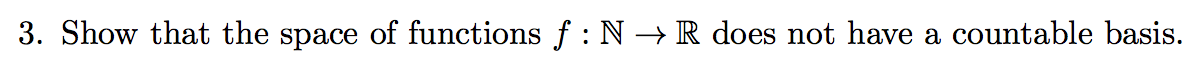
\includegraphics[width=400pt]{img/linear-algebra-a0-1-3.png}\\
\begin{mdframed}
\end{mdframed}

\subsection*{} % 4
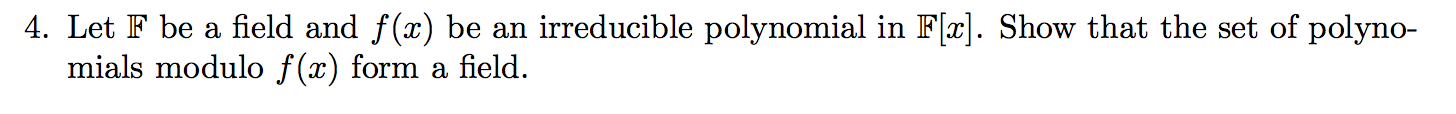
\includegraphics[width=400pt]{img/linear-algebra-a0-1-4.png}\\
\begin{mdframed}
\end{mdframed}

\subsection*{} % 5
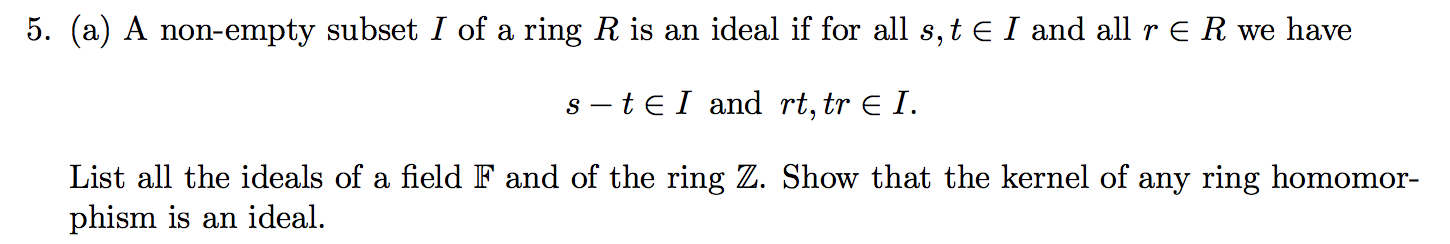
\includegraphics[width=400pt]{img/linear-algebra-a0-1-5-a.png}\\
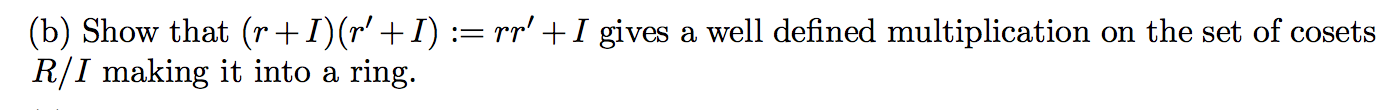
\includegraphics[width=400pt]{img/linear-algebra-a0-1-5-b.png}\\
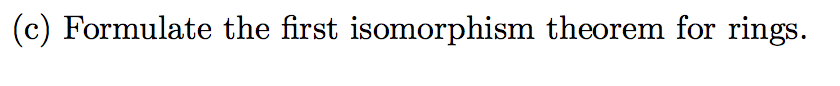
\includegraphics[width=280pt]{img/linear-algebra-a0-1-5-c.png}\\
\begin{mdframed}
\end{mdframed}

\subsection*{} % 6
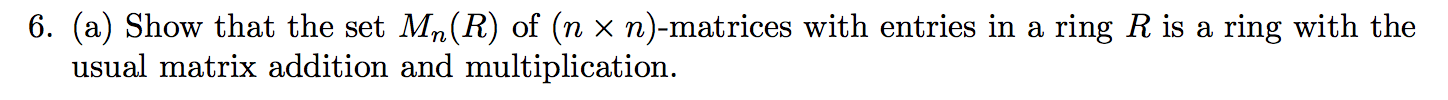
\includegraphics[width=400pt]{img/linear-algebra-a0-1-6-a.png}\\
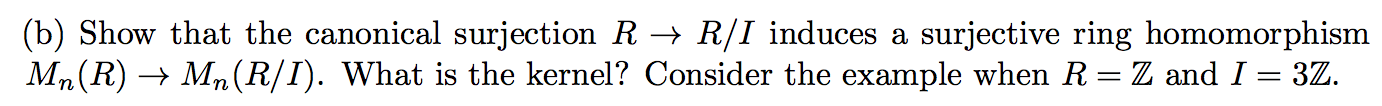
\includegraphics[width=400pt]{img/linear-algebra-a0-1-6-b.png}\\

\includegraphics[width=350pt]{img/linear-algebra-a0-1-6-c.png}\\
\begin{mdframed}
\end{mdframed}

\subsection*{} % 7
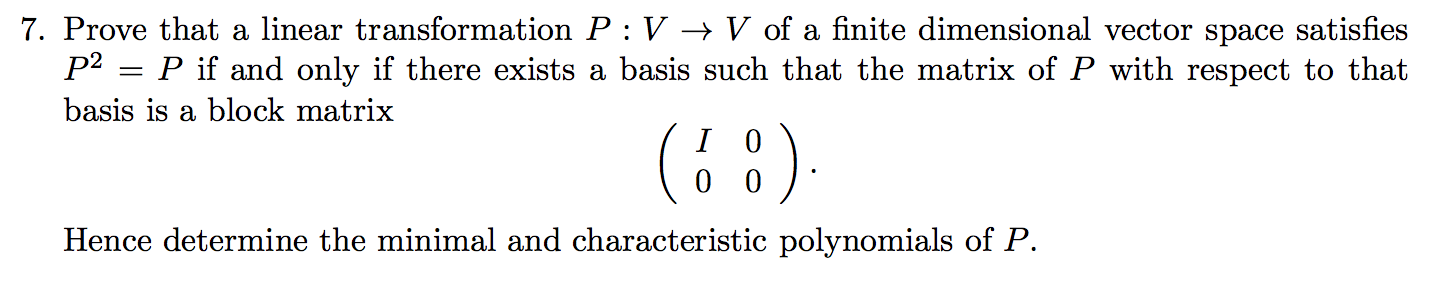
\includegraphics[width=400pt]{img/linear-algebra-a0-1-7.png}\\
\begin{mdframed}
\end{mdframed}

\subsection*{} % 8
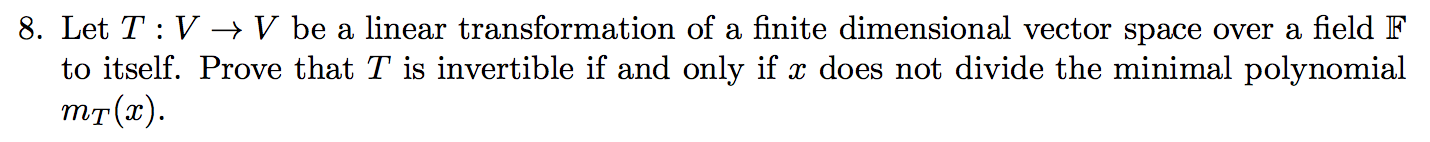
\includegraphics[width=400pt]{img/linear-algebra-a0-1-8.png}\\
\begin{mdframed}
\end{mdframed}

\subsection*{} % 9
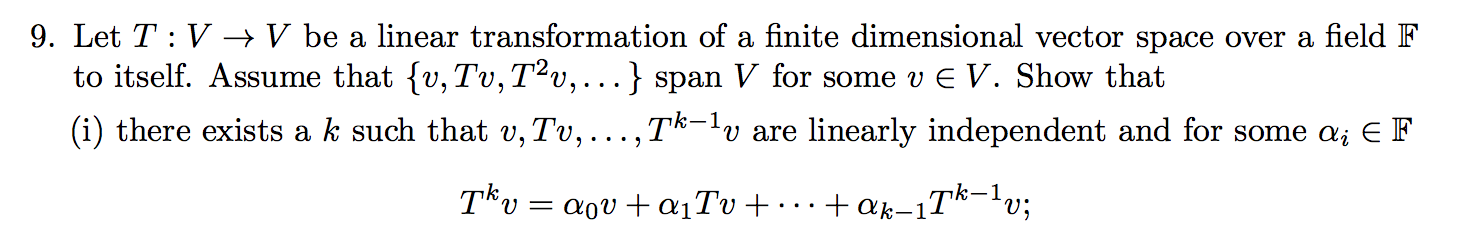
\includegraphics[width=400pt]{img/linear-algebra-a0-1-9-a.png}\\
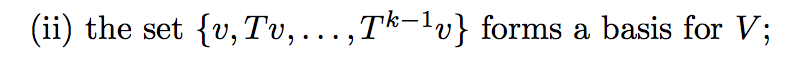
\includegraphics[width=280pt]{img/linear-algebra-a0-1-9-b.png}\\
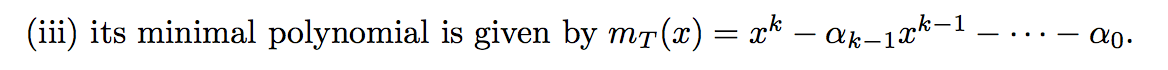
\includegraphics[width=400pt]{img/linear-algebra-a0-1-9-c.png}\\

\includegraphics[width=270pt]{img/linear-algebra-a0-1-9-d.png}\\
\begin{mdframed}
\end{mdframed}

\end{document}
